% !TEX program = pdflatex
\documentclass{beamer}
% \documentclass{beamer}

\usetheme{Madrid}
\usecolortheme{default}

\definecolor{THUpurple}{RGB}{102,8,116}

\usepackage{amsmath}
\usepackage{caption}
\usepackage{listings}
\usepackage{lmodern}
\usepackage{xcolor}
\lstset{language=Python,keywordstyle={\bfseries \color{blue}}}
\usepackage{pdfpages}
\usepackage{makecell}
\usepackage[EULERGREEK]{sansmath}
\usepackage{tikz}
\usefonttheme[onlymath]{serif}

\newcommand{\ud}{\mathrm{d}}
\newcommand{\mev}{\mathrm{MeV}}
\newcommand{\gev}{\mathrm{GeV}}

\setbeamercolor{structure}{fg=THUpurple}
\setbeamersize{text margin left=10mm,text margin right=10mm}
% \setlength{\belowcaptionskip}{-2mm}
\title[Waveform Analysis]{A Survey of PMT Waveform Analysis Methods}
\author[Dacheng Xu]{Dacheng Xu \\ [4mm] In cooperation with \and Erjin Bao \and Yiyang Wu  \\ Benda Xu \and Yu Xu \and Geliang Zhang \\ [4mm] \includegraphics[height=2cm]{img/Tsinghua_University_Logo.png} \hspace{6mm} \includegraphics[height=2cm]{img/Js.png} \\ [4mm] at DANCE Machine Learning Workshop 2020 \\ [-8mm]}
\date[DANCE]{August 4, 2020}

\AtBeginSection[]
{
    \begin{frame}[noframenumbering]
        \frametitle{Outline}
        \thispagestyle{empty}
        \tableofcontents[currentsection]
    \end{frame}
}

\begin{document}
\captionsetup[figure]{labelfont={bf},name={Fig}}
\frame{\titlepage}

\begin{frame}[noframenumbering]
\frametitle{Outline}
\thispagestyle{empty}
\tableofcontents
\end{frame}

\section{Motivation}
\begin{frame}
\setlength{\abovecaptionskip}{0mm}
\setlength{\belowcaptionskip}{0mm}
\setcounter{page}{0}
\frametitle{CJPL}
\begin{columns}
\column{0.5\textwidth}
\begin{figure}
    \centering
    \caption{China JinPing Underground Laboratory}
    \includegraphics[width=1.0\linewidth]{img/WorldMap.jpg}
\end{figure}
\column{0.5\textwidth}
\begin{figure}
    \centering
    \caption{Total intensity of $\mu$ at different underground sites}
    \includegraphics[width=1.0\linewidth]{img/muonlab.pdf}
\end{figure}
\end{columns}
\begin{itemize}
    \item Overburden $\sim2400\mathrm{m}$
    \item Extremely low cosmic-ray $\mu$ flux
    \item Low reactor neutrino flux
    \item Ideal site of low background physics research
\end{itemize}
\end{frame}

\begin{frame}
\frametitle{Jinping Neutrino Experiment}
\setlength{\abovecaptionskip}{-2mm}
\vspace{-4mm}
\begin{columns}
\column{0.33\textwidth}
\begin{center}
    Ongoing
\end{center}
\begin{figure}
    \centering
    \caption{1-ton prototype}
    \includegraphics[width=0.6\linewidth]{img/prototype.jpeg}
\end{figure}
\column{0.34\textwidth}
\begin{center}
    Next
\end{center}
\begin{figure}
    \centering
    \caption{$\sim$100t detector}
    \includegraphics[width=0.6\linewidth]{img/100tondetector.png}
\end{figure}
\column{0.33\textwidth}
\begin{center}
    Future
\end{center}
\begin{figure}
    \centering
    \caption{$\sim$5000t detector}
    \includegraphics[width=0.6\linewidth]{img/DetectoratJinping.jpg}
\end{figure}
\end{columns}
\end{frame}

\begin{frame}
\frametitle{Neutrino Detector}
\begin{columns}
\column{0.5\textwidth}
\begin{figure}
    \centering
    \caption{Future Detector at Jinping}
    \includegraphics[width=1.0\linewidth]{img/DetectoratJinping.jpg}
\end{figure}
\column{0.5\textwidth}
\begin{itemize}
    \item Study neutrino property based on interaction
    \item Study interaction based on light
    \item PMT: extremely sensitive detectors of light
\end{itemize}
\end{columns}
\end{frame}

\begin{frame}
\frametitle{Photomultiplier Tube}
\setlength{\abovecaptionskip}{0mm}
\setlength{\belowcaptionskip}{0mm}
\begin{columns}
\column{0.6\textwidth}
\begin{figure}
    \centering
    \caption{PMT}
    \includegraphics[width=0.3\linewidth]{img/PMT.png}
\end{figure}
\begin{figure}
    \centering
    \caption{PMT Single PE response}
    \includegraphics[width=0.9\linewidth]{img/pmtspe.png}
\end{figure}
\column{0.4\textwidth}
\begin{center}
    3 individual processes:
\end{center}
\begin{itemize}
    \item Photon-Electron conversion
    \item Electron collection
    \item Amplify
\end{itemize}
\end{columns}
\end{frame}

\begin{frame}
\frametitle{Naive Method}
\hspace{4mm}Naively, when handling PMT waveforms, we record:
\begin{itemize}
    \item First HitTime
    \item Integration of Waveform (Charge)
\end{itemize}
\begin{figure}
    \centering
    % \caption{Traditional Recorded Waveform}
    \includegraphics[width=0.8\linewidth]{img/previous.png}
\end{figure}
\end{frame}

\begin{frame}
\frametitle{New Goal}
\begin{itemize}
    \item Extract All Detailed Photon Information in 1 Window
    \item Including: HitTime (The time when electron hit first dynode) \& Charge or PEnumber
\end{itemize}
\begin{figure}
    \centering
    % \caption{Traditional Recorded Waveform}
    \includegraphics[width=0.8\linewidth]{img/goal.png}
\end{figure}
\end{frame}

\begin{frame}
\frametitle{Charge vs PEnum}
\setlength{\abovecaptionskip}{0mm}
\setlength{\belowcaptionskip}{0mm}
\begin{figure}
    \centering
    \caption{10 Single PE response}
    \includegraphics[width=0.8\linewidth]{img/spewaves.png}
\end{figure}
\vspace{-4mm}
\hspace{8mm}Difference charge for one photon electron
\end{frame}

\section{Wasserstein Distance}
\begin{frame}
\frametitle{Measurement of difference}
\begin{center}
    The difference between Reconstruction Result \& Truth?
\end{center}
\end{frame}

\begin{frame}
\frametitle{Familiar Distances}
\begin{columns}
\column{0.3\textwidth}
\begin{itemize}
    \item $L_{1}$ : $\int|p-q|$
    \item $L_{2}$ : $\int(p-q)^{2}$
    \item $\chi^{2}$ : $\int\frac{(p-q)^{2}}{q}$
    \item $\cdots$
\end{itemize}
\column{0.7\textwidth}
Shortcoming:
\begin{itemize}
    \item Cannot compare discrete distribution with continuous distribution
    \item Ignore the geometry of space
\end{itemize}
\begin{figure}
    \centering
    \includegraphics[width=1.0\linewidth]{img/tab.png}
\end{figure}
\end{columns}
\end{frame}

% !TEX program = pdflatex
\documentclass{beamer}

% \usetheme{Madrid}
\usepackage{amsmath,mathrsfs}
\usepackage{tikz}

\tikzset{elegant/.style={smooth,thick,samples=50,cyan}}
\tikzset{eaxis/.style={->,>=stealth}}

\begin{document}
\begin{frame}
    \resizebox{\textwidth}{!}{
    \begin{tikzpicture}
        % draw the axis
        \draw[eaxis] (-1.5,0) -- (4,0) node[below] {$x$};
        % draw the function (piecewise)
        \draw[elegant,domain=-1.5:3.5] plot(\x,{pow(e,-(\x)^2*4)*2}) node [anchor=east] at (0,2) {$\mu(x)$};
        \draw[elegant,orange,domain=-1.5:3.5] plot(\x,{pow(e,-(\x-1)^2)}) node [anchor=west] at (1,1) {$\nu(x)$};
        
        \draw[->] (0,2) to[out=0, in=90] (1,1);
        \node at (1.4,1.9)  {\tiny$W(\mu(x),\nu(x))$};
    \end{tikzpicture}
    }
\end{frame}
\begin{frame}
    \resizebox{\textwidth}{!}{
    \begin{tikzpicture}
        % draw the axis
        \draw[eaxis] (-1.5,0) -- (4,0) node[below] {$x$};
        % draw the function (piecewise)
        \draw[elegant,domain=-1.5:3.5] plot(\x,{pow(e,-(\x)^2*4)*2});
        \draw[elegant,orange,domain=-1.5:3.5] plot(\x,{pow(e,-(\x-1)^2)});
        
        \draw[fill=red] (-0.15,0.3) rectangle (-0.05,0.9) node [anchor=east] (block1) {};
        \draw[fill=green] (-0.15,0.9) rectangle (-0.05,1.9) node [anchor=east] (block2) {};
        \draw[fill=red] (0.65,0.3) rectangle (0.75,0.9) node (block3) {};
        \draw[fill=green] (0.85,0.09) rectangle (0.95,0.99) node (block4) {};
        
        \draw (-0.1,0.3) -- (-0.1,0) node [anchor=north] {\tiny$x$};
        \draw (0.7,0.3) -- (0.7,0) node [anchor=north] {\tiny$y_1$};
        \draw (0.9,0.1) -- (0.9,0) node [anchor=north] {\tiny$y_2$};
        
        \draw[red,->] (block1) -- (block3);
        \draw[green,->] (block2) to[out=0, in=120] (block4);
    \end{tikzpicture}
    }
\end{frame}

\begin{frame}
    \resizebox{\textwidth}{!}{
    \begin{tikzpicture}
        % draw the axis
        \draw[eaxis] (-1.5,0) -- (4,0) node[below] {$x$};
        % draw the function (piecewise)
        \draw[elegant,domain=-1.5:3.5] plot(\x,{pow(e,-(\x)^2*4)*2});
        \draw[elegant,orange,domain=-1.5:3.5] plot(\x,{pow(e,-(\x-1)^2)});
        
        \draw[fill=red] (-0.15,0.3) rectangle (-0.05,0.9) node [anchor=east] (block1) {};
        \draw[<->] (-0.2,0.3) -- (-0.2,0.9);
        \node [anchor=east] at (-0.1,0.6) {\tiny$\pi(x,y_1)\Delta y_1$};
        \draw[fill=green] (-0.15,0.9) rectangle (-0.05,1.9) node [anchor=east] (block2) {};
        \draw[<->] (-0.2,0.9) -- (-0.2,1.9);
        \node [anchor=east] at (-0.1,1.4) {\tiny$\pi(x,y_2)\Delta y_2$};
        \draw[fill=red] (0.65,0.3) rectangle (0.75,0.9) node (block3) {};
        \draw[fill=green] (0.85,0.09) rectangle (0.95,0.99) node (block4) {};
        
        \draw (-0.1,0.3) -- (-0.1,0) node [anchor=north] {\tiny$x$};
        \draw (0.7,0.3) -- (0.7,0) node [anchor=north] {\tiny$y_1$};
        \draw (0.9,0.1) -- (0.9,0) node [anchor=north] {\tiny$y_2$};
        
        \draw[red,->] (block1) -- (block3);
        \node at (0.35,1.05)  {\tiny$d(x,y_1)$};
        \draw[green,->] (block2) to[out=0, in=120] (block4);
        \node at (0.6,1.6)  {\tiny$d(x,y_2)$};
    \end{tikzpicture}
    }
\pause
\begin{equation*}
    \begin{aligned}
        &\pi(x,y_1)\Delta y_1 + \pi(x,y_1)\Delta y_2 = \mu(x) - \nu(x) \\
        &\Delta W=\pi(x,y_1)\Delta x\Delta y_1 d(x,y_1) + \pi(x,y_2)\Delta x\Delta y_2 d(x,y_2) \\
    \end{aligned}
\end{equation*}
\pause
\begin{equation*}
    \begin{aligned}
    \therefore &\int \pi(x,y)\mathrm{d}y = \mu(x),\ \ \ \ \int \pi(x,y)\mathrm{d}x = \nu(y) \\
        &W(\mu(x),\nu(x))|_{\pi=\pi(x,y)} = \iint \pi(x,y)d(x,y)\mathrm{d}x\mathrm{d}y = \int d(x,y)\mathrm{d}\pi(x,y)\\
    \end{aligned}
\end{equation*}
\end{frame}
\begin{frame}
    \resizebox{\textwidth}{!}{
    \begin{tikzpicture}
        % draw the axis
        \draw[eaxis] (-1.5,0) -- (4,0) node[below] {$x$};
        % draw the function (piecewise)
        \draw[elegant,domain=-1.5:3.5] plot(\x,{pow(e,-(\x)^2*4)*2});
        \draw[elegant,orange,domain=-1.5:3.5] plot(\x,{pow(e,-(\x-1)^2)});
        
        \draw[fill=red] (-0.15,0.3) rectangle (-0.05,0.9) node [anchor=east] (block1) {};
        \draw[<->] (-0.2,0.3) -- (-0.2,0.9);
        \node [anchor=east] at (-0.1,0.6) {\tiny$\pi(x,y_1)\Delta y_1$};
        \draw[fill=green] (-0.15,0.9) rectangle (-0.05,1.9) node [anchor=east] (block2) {};
        \draw[<->] (-0.2,0.9) -- (-0.2,1.9);
        \node [anchor=east] at (-0.1,1.4) {\tiny$\pi(x,y_2)\Delta y_2$};
        \draw[fill=red] (0.65,0.3) rectangle (0.75,0.9) node (block3) {};
        \draw[fill=green] (0.85,0.09) rectangle (0.95,0.99) node (block4) {};
        
        \draw (-0.1,0.3) -- (-0.1,0) node [anchor=north] {\tiny$x$};
        \draw (0.7,0.3) -- (0.7,0) node [anchor=north] {\tiny$y_1$};
        \draw (0.9,0.1) -- (0.9,0) node [anchor=north] {\tiny$y_2$};
        
        \draw[red,->] (block1) -- (block3);
        \node at (0.35,1.05)  {\tiny$d(x,y_1)$};
        \draw[green,->] (block2) to[out=0, in=120] (block4);
        \node at (0.6,1.6)  {\tiny$d(x,y_2)$};
    \end{tikzpicture}
    }
    Choosing the best transportaion $\pi(x,y) \in \Pi(\mu,\nu)$:
\begin{equation*}
    \begin{aligned}
        \mathrm{Wasserstein}(\mu(x),\nu(x)) &= \inf_{\pi \in \Pi(\mu,\nu)} W(\mu(x),\nu(x))|_{\pi=\pi(x,y)} \\
        &=\inf_{\pi \in \Pi(\mu,\nu)}\int d(x,y)\mathrm{d}\pi(x,y)\\
    \end{aligned}
\end{equation*}
\end{frame}   
\end{document}
        % 建立相对坐标系
        % \draw[help lines,xstep=.1,ystep=.1] (-1.5,0) grid (pi,2);

\begin{frame}
\frametitle{Wasserstein Distance Demo}
\setlength{\abovecaptionskip}{-2mm}
\setlength{\belowcaptionskip}{0mm}
$D_{w}=\sum|\mathrm{CDF}(a) - \mathrm{CDF}(b)|$ \\
$CDF$: Cumulative Distribution Function
\begin{columns}
\column{0.4\textwidth}
\begin{figure}
    \centering
    \includegraphics[width=1.0\linewidth]{img/a.png}
\end{figure}
\vspace{-7mm}
\begin{figure}
    \centering
    \includegraphics[width=1.0\linewidth]{img/b.png}
\end{figure}
\column{0.1\textwidth}
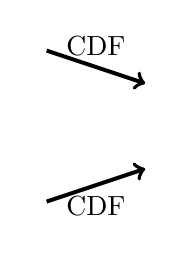
\begin{tikzpicture}
    \node[] at (-2.5, 1) (a1) {};
    \node[] at (-1, 0.5) (a2) {};
    \node[] at (-2.5, -1) (b1) {};
    \node[] at (-1, -0.5) (b2) {};
    \draw [->, line width=0.5mm] (a1) -- node[anchor=south] {CDF} (a2);
    \draw [->, line width=0.5mm] (b1) -- node[anchor=north] {CDF} (b2);
\end{tikzpicture}
\column{0.5\textwidth}
\vspace{2mm}\begin{figure}
    \centering
    \includegraphics[width=1.0\linewidth]{img/ab.png}
\end{figure}
\rightline{W-dist = $1.8\mathrm{ns}$}
\end{columns}
This definition of distance is equivalent to Wasserstein Distance
\end{frame}

\section{Methods}

\begin{frame}
\frametitle{Input \& Output, Loss}
\begin{columns}
\column{0.4\textwidth}
\hspace{4mm}Input \& Output:
\begin{itemize}
    \item Input: Pedestal deduced PMT waveform
    \item Output: Weight (Charge or PEnumber) sequence
\end{itemize}
\column{0.6\textwidth}
\setlength{\abovecaptionskip}{-2mm}
\setlength{\belowcaptionskip}{0mm}
\begin{figure}
    \centering
    \includegraphics[width=0.9\linewidth]{img/wave.png}
    \includegraphics[width=0.9\linewidth]{img/charge.png}
\end{figure}
\end{columns}
\end{frame}

\begin{frame}
\frametitle{Data Sample}
PEpos \& PEnum is the count of HitTime
\begin{columns}
\column{0.6\textwidth}
\begin{figure}
    \centering
    \caption{PEpos Histogram}
    \includegraphics[width=1.0\linewidth]{img/pepos.png}
\end{figure}
\column{0.4\textwidth}
\begin{figure}
    \centering
    \caption{Data Structure}
    \includegraphics[width=1.0\linewidth]{img/dataset.png}
\end{figure}
\end{columns}
\end{frame}

\begin{frame}
\frametitle{Find Peak}
\begin{figure}
    \centering
    \caption{Find Peak Method Demo, W-dist = 4.02}
    \includegraphics[width=0.9\linewidth]{img/findpeak.png}
\end{figure}
\vspace{-4mm}
\begin{center}
    Average W-dist = 10.70 (Charge), 11.62 (PEnum)
\end{center}
\end{frame}

\begin{frame}
\frametitle{Waveform Shift}
\begin{figure}
    \centering
    \caption{Waveform Shift Method Demo, W-dist = 10.75}
    \includegraphics[width=0.9\linewidth]{img/threshold.png}
\end{figure}
\vspace{-4mm}
\begin{center}
    Average W-dist = 3.67 (Charge), 4.69 (PEnum)
\end{center}
\end{frame}

\begin{frame}
\frametitle{Fast Fourier Transform}
\begin{columns}
\column{0.6\textwidth}
\begin{figure}
    \centering
    \caption{Fast Fourier Transform Demo, W-dist = 1.63}
    \includegraphics[width=1.0\linewidth]{img/fftrans.png}
\end{figure}
\vspace{-4mm}
\begin{center}
    Average W-dist = 1.44 (Charge), 3.08 (PEnum)
\end{center}
\column{0.4\textwidth}
\begin{enumerate}
    \item FFT of Waveform \& Single PE response
    \item Rectangular filter of FFT(Waveform)
    \item FFT(Charge) = FFT(Waveform) / FFT(SPE)
    \item IFFT of FFT(Charge)
\end{enumerate}
\end{columns}
\end{frame}

\begin{frame}
\frametitle{Lucy Deconvolution}
\begin{columns}
\column{0.6\textwidth}
\begin{figure}
    \centering
    \caption{Lucy Deconvolution Demo, W-dist = 1.25}
    \includegraphics[width=1.0\linewidth]{img/lucyddm.png}
\end{figure}
\vspace{-4mm}
\begin{center}
    Average W-dist = 0.93 (Charge), 2.74 (PEnum)
\end{center}
\column{0.4\textwidth}
\begin{enumerate}
    \item Lucy-Richardson deconvolution
    \item A nonlinear iterative method
    \item Prohibit Charge $<$ 0
\end{enumerate}
\end{columns}
\end{frame}

\begin{frame}
\frametitle{CNN Structure}
\begin{columns}
\column{0.35\textwidth}
\begin{figure}[H]
    \centering
    \caption{CNN Structure}
    \includegraphics[width=0.8\textwidth]{img/model.png}
\end{figure}
\column{0.65\textwidth}
\lstinputlisting[language=Python, basicstyle=\tiny]{CNN}
\end{columns}
\end{frame}

\begin{frame}
\frametitle{Training Process}
\begin{columns}
\column{0.35\textwidth}
\begin{itemize}
    \item Train CNN by each Channel (30PMTs)
    \item $\sim$450k waveform for each Channel
    \item epoch = 36
    \item Learning rate = $0.01$
\end{itemize}
\column{0.65\textwidth}
\begin{figure}
    \centering
    \caption{Loss variation during training (Channel 5)}
    \includegraphics[width=1.0\linewidth]{img/epoch.png}
\end{figure}
\end{columns}
\end{frame}

\begin{frame}
\frametitle{CNN Result}
\begin{figure}
    \centering
    \caption{CNN PEnum Result Histogram}
    \includegraphics[width=0.85\linewidth]{img/takarapenumhist.png}
\end{figure}
\begin{center}
    Average W-dist = 2.25 (Charge), 0.76 (PEnum)
\end{center}
\end{frame}

\begin{frame}
\frametitle{CNN Result}
\setlength{\abovecaptionskip}{0mm}
\setlength{\belowcaptionskip}{0mm}
\begin{figure}
    \centering
    \caption{CNN PEnum W-dist vs PEnum}
    \includegraphics[width=0.65\linewidth]{img/takarapenumstats.png}
\end{figure}
\end{frame}

\begin{frame}
\frametitle{Single PE Model}
\begin{figure}
    \centering
    \caption{Single PE Model}
    \includegraphics[width=0.9\linewidth]{img/spe.png}
\end{figure}
\end{frame}

\begin{frame}
\frametitle{Fitting (Match Pursuit) Process}
\begin{itemize}
    \item Fitting parameter: Weight in each HitTime
    \item loss is Residual sum squares of Waveform
    \item Loss = $\sum(Wave_{recon}-Wave_{truth})^{2}$
    \item using \lstinline{scipy.optimize.fmin_l_bfgs_b}
\end{itemize}
\setlength{\abovecaptionskip}{0mm}
\setlength{\belowcaptionskip}{0mm}
\begin{figure}
    \centering
    \caption{Fitting Demo}
    \includegraphics[width=0.78\linewidth]{img/demo.png}
\end{figure}
\end{frame}

\begin{frame}
\frametitle{Fitting Result}
\begin{figure}
    \centering
    \caption{Fitting Charge Result Histogram}
    \includegraphics[width=0.85\linewidth]{img/xiaopeipchargehist.png}
\end{figure}
\begin{center}
    Average W-dist = 0.54 (Charge), 2.46 (PEnum)
\end{center}
\end{frame}

\begin{frame}
\frametitle{Fitting Result}
\setlength{\abovecaptionskip}{0mm}
\setlength{\belowcaptionskip}{0mm}
\begin{figure}
    \centering
    \caption{Fitting Charge W-dist vs PEpos}
    \includegraphics[width=0.65\linewidth]{img/xiaopeipchargestats.png}
\end{figure}
\end{frame}

\section{Result}
\begin{frame}
\frametitle{Distances}
\begin{figure}
    \centering
    \caption{Distances of methods, error bar 10 - 90 percentile (Charge)}
    \includegraphics[width=1.0\linewidth]{img/summarycharge.png}
\end{figure}
\end{frame}

\begin{frame}
\frametitle{Distances}
\begin{figure}
    \centering
    \caption{Distances of methods, error bar 10 - 90 percentile (PEnum)}
    \includegraphics[width=1.0\linewidth]{img/summarypenum.png}
\end{figure}
\end{frame}

\begin{frame}
\frametitle{Efficiency}
\begin{table}
    \centering
    \caption{Reconstruction Efficiency}
    \begin{tabular}{c|c|c}
        \hline
        &  & Performance \\
        \hline
        CNN & Charge & 6.0s/$10^{5}$Wf(1gpu) \\
        \hline
        CNN & PEnum & 6.0s/$10^{5}$Wf(1gpu)\\
        \hline
        Fitting & Charge & 2000s/$10^{5}$Wf(50cpu) \\
        \hline
        Fitting & PEnum & 2000s/$10^{5}$Wf(50cpu) \\
        \hline
    \end{tabular}
\end{table}
\end{frame}

\section{Summary \& Outlook}
\begin{frame}
\frametitle{Summary \& Outlook}
\begin{itemize}
    \item We developed several representative methods to extract photon information hidden in PMT waveform
    \item These methods will improve the accuracy of following-up Event reconstruction
    \item We are working on applying and connecting these methods to Event reconstruction
\end{itemize}
\end{frame}

\appendix
\section{Backup}
\begin{frame}[noframenumbering]
\thispagestyle{empty}
\frametitle{Backup - Poisson Distance \& Charge Diff}
\hspace{4mm}Poisson Distance is used \textbf{only} when reconstruct PEnumber
\begin{itemize}
    \item $Q = \sum PEnumber_{truth_i}; q = \sum PEnumber_{recon_i}$
    \item $D_{p} = |Q-q|*\mathrm{Poisson}(Q|Q)$
\end{itemize}
\hspace{4mm}Charge Diff is used \textbf{only} when reconstruct Charge
\end{frame}

\begin{frame}[noframenumbering]
\thispagestyle{empty}
\frametitle{Backup - PEpos vs PEnum}
\begin{columns}
\column{0.5\textwidth}
\begin{figure}
    \centering
    \includegraphics[width=1.0\linewidth]{img/pepos.png}
\end{figure}
\column{0.5\textwidth}
\begin{figure}
    \centering
    \includegraphics[width=1.0\linewidth]{img/penum.png}
\end{figure}
\end{columns}
\end{frame}

\begin{frame}[noframenumbering]
\thispagestyle{empty}
\frametitle{Backup - Fitting Result}
\begin{figure}
    \centering
    \caption{Fitting PEnum Result Histogram}
    \includegraphics[width=0.85\linewidth]{img/xiaopeippenumhist.png}
\end{figure}
\end{frame}

\begin{frame}[noframenumbering]
\thispagestyle{empty}
\frametitle{Backup - Fitting Result}
\setlength{\abovecaptionskip}{0mm}
\setlength{\belowcaptionskip}{0mm}
\begin{figure}
    \centering
    \caption{Fitting PEnum W-dist vs PEpos}
    \includegraphics[width=0.65\linewidth]{img/xiaopeippenumstats.png}
\end{figure}
\end{frame}

\begin{frame}[noframenumbering]
\thispagestyle{empty}
\frametitle{Backup - CNN Result}
\begin{figure}
    \centering
    \caption{CNN Charge Result Histogram}
    \includegraphics[width=0.85\linewidth]{img/takarachargehist.png}
\end{figure}
\end{frame}

\begin{frame}[noframenumbering]
\thispagestyle{empty}
\frametitle{Backup - CNN Result}
\setlength{\abovecaptionskip}{0mm}
\setlength{\belowcaptionskip}{0mm}
\begin{figure}
    \centering
    \caption{CNN Charge W-dist vs PEpos}
    \includegraphics[width=0.65\linewidth]{img/takarachargestats.png}
\end{figure}
\end{frame}

\begin{frame}[noframenumbering]
\thispagestyle{empty}
\frametitle{Backup - Large W-dist}
\begin{figure}
    \centering
    \includegraphics[width=1.0\linewidth]{img/demoe15231c15.png}
\end{figure}
\end{frame}

\begin{frame}[noframenumbering]
\thispagestyle{empty}
\frametitle{Backup - Large W-dist}
\begin{figure}
    \centering
    \includegraphics[width=1.0\linewidth]{img/demoe22746c2.png}
\end{figure}
\end{frame}

\end{document}